%% FEUP THESIS STYLE for LaTeX2e
%% how to use feupteses (English version)
%%
%% FEUP, JCL & JCF, 31 July 2012
%%
%% PLEASE send improvements to jlopes at fe.up.pt and to jcf at fe.up.pt
%%

%%========================================
%% Commands: pdflatex tese
%%           bibtex tese
%%           makeindex tese (only if creating an index) 
%%           pdflatex tese
%% Alternative:
%%          latexmk -pdf tese.tex
%%========================================

\documentclass[11pt,a4paper,twoside,openright]{report}

%% For iso-8859-1 (latin1), comment next line and uncomment the second line
\usepackage[utf8]{inputenc}
%\usepackage[latin1]{inputenc}
\usepackage[portuguese,english]{babel}

%% English version

%% MIEIC options
\usepackage[mieic]{feupteses}
%\usepackage[mieic,juri]{feupteses}
%\usepackage[mieic,final]{feupteses}
%\usepackage[mieic,final,onpaper]{feupteses}

%% Additional options for feupteses.sty: 
%% - onpaper: links are not shown (for paper versions)
%% - backrefs: include back references from bibliography to citation place

%% Uncomment the next lines if side by side graphics used
%\usepackage[lofdepth,lotdepth]{subfig}
%\usepackage{graphicx}
%\usepackage{float}

%% Include color package
\usepackage{color}
\definecolor{cloudwhite}{cmyk}{0,0,0,0.025}

%% Include source-code listings package
\usepackage{listings}
\lstset{ %
 language=C,                        % choose the language of the code
 basicstyle=\footnotesize\ttfamily,
 keywordstyle=\bfseries,
 numbers=left,                      % where to put the line-numbers
 numberstyle=\scriptsize\texttt,    % the size of the fonts that are used for the line-numbers
 stepnumber=1,                      % the step between two line-numbers. If it's 1 each line will be numbered
 numbersep=8pt,                     % how far the line-numbers are from the code
 frame=tb,
 float=htb,
 aboveskip=8mm,
 belowskip=4mm,
 backgroundcolor=\color{cloudwhite},
 showspaces=false,                  % show spaces adding particular underscores
 showstringspaces=false,            % underline spaces within strings
 showtabs=false,                    % show tabs within strings adding particular underscores
 tabsize=2,	                    % sets default tabsize to 2 spaces
 captionpos=b,                      % sets the caption-position to bottom
 breaklines=true,                   % sets automatic line breaking
 breakatwhitespace=false,           % sets if automatic breaks should only happen at whitespace
 escapeinside={\%*}{*)},            % if you want to add a comment within your code
 morekeywords={*,var,template,new}  % if you want to add more keywords to the set
}

%% Uncomment to create an index (at the end of the document)
%\makeindex

%% Path to the figures directory
%% TIP: use folder ``figures'' to keep all your figures
\graphicspath{{figures/}}

%%----------------------------------------
%% TIP: if you want to define more macros, use an external file to keep them
%some macro definitions

% format
\newcommand{\class}[1]{{\normalfont\slshape #1\/}}

% entities
\newcommand{\Feup}{Faculdade de Engenharia da Universidade do Porto}

\newcommand{\svg}{\class{SVG}}
\newcommand{\scada}{\class{SCADA}}
\newcommand{\scadadms}{\class{SCADA/DMS}}

%%----------------------------------------

%%========================================
%% Start of document
%%========================================
\begin{document}

%%----------------------------------------
%% Information about the work
%%----------------------------------------
\title{Engenharia Reversa de Padrões de Interação}
\author{Clara Sacramento}

%% Uncomment next line for date of submission
%\thesisdate{July 31, 2008}

%%Uncomment next line for copyright text if used
%\copyrightnotice{Name of the Author, 2008}

\supervisor{Supervisor}{Ana Paiva (PhD)}

%% Uncomment next line if necessary
%\supervisor{Second Supervisor}{Name of the Supervisor}

%% Uncomment committee stuff in the final version if used
%\committeetext{Approved in oral examination by the committee:}
%\committeemember{Chair}{Doctor Name of the President}
%\committeemember{External Examiner}{Doctor Name of the Examiner}
%\committeemember{Supervisor}{Doctor Name of the Supervisor}
%\signature

%% Specify cover logo (in folder ``figures'')
\logo{uporto-feup.pdf}

%% Uncomment next line for additional text  below the author's name (front page)
%\additionalfronttext{Preparação da Dissertação}

%%----------------------------------------
%% Preliminary materials
%%----------------------------------------

% remove unnecssary \include{} commands
\begin{Prolog}
  \chapter*{}

This work is financed by the ERDF - European Regional Development Fund through the COMPETE Programme (operational programme for competitiveness) and by National Funds through the FCT - Fundação para a Ciência e a Tecnologia (Portuguese Foundation for Science and Technology) within project FCOMP-01-0124-FEDER-020554.

\begin{figure}[!b]
  \begin{center}
    \leavevmode
    
\includegraphics[width=\textwidth]{acks}
    \label{fig:arch}
  \end{center}
\end{figure}  % the FCT
  \chapter*{Abstract}
A great deal of effort in model-based testing is related to the creation of the model. In addition, the model itself, while a powerful tool of abstraction, can have conceptual errors, introduced by the tester. These problems can be reduced by generating those models automatically. This dissertation presents a dynamic reverse engineering approach that aims to extract part of the model of an existing Web application through the identification of User Interface (UI) patterns. This reverse engineering approach explores automatically any Web application, records information related to the interaction, analyzes the gathered information, tokenizes it, and infers the existing UI patterns via syntactical analyzing. After complemented with additional information and validated, the model extracted is the input for the Pattern-Based Graphical User Interface Testing (PBGT) approach for testing existing web application under analysis.

First the theme developed during the course of the dissertation is introduced, starting by defining the context and issue at hand and describing the goals of this dissertation. Afterwards we present a literary review on reverse engineering approaches, approaches that infer patterns from Web applications, and data mining algorithms and tools relevant to the problem. We explain the approach in detail, present a case study, and lastly, we present the conclusions taken from the work.

\chapter*{Resumo}
\begin{otherlanguage}{portuguese}
Grande parte do esforço despendido em testes baseados num modelo está relacionado com a criação do modelo. Além disso, o modelo, mesmo sendo uma ferramenta poderosa de abstração, pode ter erros conceptuais introduzidos pelo testador. Esses problemas podem ser reduzidos ao gerar esses modelos automaticamente. Esta dissertação apresenta uma abordagem de engenharia reversa dinâmica que pretende extrair parte do modelo de uma aplicação Web a testar, diretamente da sua interface gráfica, através da identificação de padrões de interface de utilizador (\textit{UI Patterns}). Esta abordagem de engenharia reversa explora automaticamente qualquer aplicação Web, guarda informação relacionada com a interação, analisa a informação guardada, analisa-a lexicalmente, e infere padrões através de análise sintáctica. Após ser complementado com informação adicional e validado, o modelo resultante serve de entrada para a abordagem de Teste de GUIs baseado em Padrões (PBGT), para testar a aplicação Web sobre análise.

Primeiro o tema desenvolvido no decorrer da dissertação é introduzido, começando por definir o seu contexto, motivação e objectivos. Depois é apresentada uma revisão bibliográfica de abordagens que usam engenharia reversa e abordagens que inferem padrões de aplicações Web.  A abordagem desenvolvida é apresentada em detalhe, é apresentado um caso de estudo, e finalmente são apresentadas as conclusões do trabalho realizado.
\end{otherlanguage} % the abstract
  \chapter*{Acknowledgements}

First of all, I would like to thank my supervisor, Ana Paiva, from the Faculty of Engineering of University of Porto, for her guidance, insight, encouragement and support during the whole masters. Our weekly moments of discussion were indispensable for the success of this work, and specially for keeping me in the right track and focused on what was important (and not what it would be cool to do).

I would also like to thank all my teachers, from the first grade to my last year in college, as without them I wouldn't have had the necessary skills to accomplish this.

My friends’ friendship has been very important to me and so I thank them for being there for me every step of the way. I would like to specially thank the members of NIAEFEUP, with a very special mention for Pedro, for all the talking, all the comfort and teasing, all the help, and the kind words in the darkest moments. Thank you for all the great moments we have spent together, and for all that we have accomplished together.

A special thank to my parents, Maria and Adelino, without whom I would not be the person I am today and would have not achieved all the great things I have in my life. Thank you for all of your love, your concern and specially your loving support. Thank you for being there for me around the clock.

And finally, a special thank to my boyfriend, Diogo. Thank you for your insight in some of my assignments. Thank you for all of your love, your friendship, the comfort you provided me, your understanding, your patience and for every time you have teased me
along the years.

%\vspace{10mm}
%\flushleft{Clara Raquel da Costa e Silva Sacramento}  % the acknowledgments
  \cleardoublepage
\thispagestyle{plain}

\vspace*{8cm}

\begin{flushright}
   \textsl{``You should be glad that bridge fell down. \\
           I was planning to build thirteen more to that same design''} \\
\vspace*{1.5cm}
           Isambard Kingdom Brunel
\end{flushright}
       % initial quotation if desired
  \cleardoublepage
  \pdfbookmark[0]{Table of Contents}{contents}
  \tableofcontents
  \cleardoublepage
  \pdfbookmark[0]{List of Figures}{figures}
  \listoffigures
  \cleardoublepage
  \pdfbookmark[0]{List of Tables}{tables}
  \listoftables
  \chapter*{Abbreviations}
\chaptermark{ABBREVIATIONS}

\begin{flushleft}
\begin{tabular}{l p{0.8\linewidth}}
FEUP	& \Feup{} \textit{(Faculdade de Engenharia da Universidade do Porto)}\\
RIA	& Rich Internet Applications \\
API	& Application Programming Interface \\
%AST	& Abstract Syntax Tree \\
DSL	& Domain Specific Language \\
AUA	& Application Under Analysis \\
CIO	& Concrete Interaction Objects \\
EFG	& Event Flow Graph \\
%FSM	& Finite State Machine \\
GUI	& Graphical User Interface \\
%MBT	& Model-Based Testing \\
SUT	& System Under Testing \\
TDD	& Test-Driven Development \\
UI	& User Interface \\
HTML	& HyperText Markup Language \\
UML	& Unified Modeling Language \\
%AUIDL	& Abstract UI Description Language \\
%HCI	& Human Computer Interaction \\
REGUI	& Reverse Engineering of Graphical User Interface \\
%V\&V	& Verification and Validation \\
XML	& eXtensible Markup Language \\
\end{tabular}
\end{flushleft}

  % the list of abbreviations used
\end{Prolog}

%%----------------------------------------
%% Body
%%----------------------------------------
\StartBody

%% TIP: use a separate file for each chapter
\chapter{Introduction} \label{chap:intro}

\section*{}

\section{Context} \label{sec:context}

Web applications are getting more and more important. Due to their stability and security against losing data, there is a growing trend to move applications towards the Web, with the most notorious examples being Google's mail and office software applications. Web applications can now handle tasks that before could only be performed by desktop applications \cite{garrett2005ajax}, like editing images or creating spreadsheet documents.

Despite the relevance that Web applications have in the community, they still suffer from a lack of standards and conventions \cite{constantine2002usage}, unlike desktop and mobile applications. This means that the same task can be implemented in many different ways, which makes automated testing difficult to accomplish and inhibits reuse of testing code. For instance, authentication (\textit{login}) failure usually triggers the appearance of an error message, but some implementations simply erase the inserted data, with no error message visible.

GUIs \textit{(Graphical User Interfaces)} of all kinds are populated with recurring behaviors that vary slightly; examples being authentication via \textit{login/password} pair and content search. These behaviors (patterns) are called User Interface (UI) patterns \cite{van2001patterns} and are recurring solutions to common design problems. Due to their widespread use, UI patterns allow users a sense of familiarity and comfort when using applications.

However, while UI patterns are familiar to users, their implementation may vary significantly. Despite this, it is possible to define generic and reusable test strategies (User Interface Test Patterns - UITP) to test those patterns. This requires a configuration process, in order to adapt the tests to different applications \cite{dalal1999model}.

Testing is an increasingly important part of any development process as it is essential to improve the trust in the quality of software. Thus, there is an ever increasing need to develop new techniques in this field. This necessity is increased by the constant improvement of development techniques.

When it comes to GUI testing, there are some applicable testing techniques \cite{memon2002gui}: \textbf{capture replay}, which requires a functional GUI; \textbf{unit testing}, which requires the manual implementation of the tests and may involve too much work in order to test all of the functionalities; \textbf{random input testing}, which is good at finding situations where the system crashes, but is not as good at finding other kinds of errors; and \textbf{model-based testing}, which enables automatic test case generation and execution, even though it requires a formal model in order to generate the test cases.

\section{Motivation and Objectives} \label{sec:goals}

As mentioned before, the focus of this dissertation is a component of a research project named PBGT (\textit{Pattern-based GUI Testing}) \cite{moreira2013pattern}. The main goal of of this project is to improve current model-based GUI testing methods and tools, contributing to conceive an effectively applicable testing approach in industry and to contribute to the construction of higher quality GUIs and software systems. One of the problems to overcome when implementing a model-based GUI testing approach is the time required to construct the model and the test case explosion problem. Choosing the right abstraction level of the model, extracting part of that model by a reverse engineering process and focusing the test cases to cover common recurrent behavior seems to be a way to solve these problems.

The proposal aims to continue the work done on PARADIGM-RE, a component of the PBGT process responsible for extracting part of the Web application model from the Web application itself via reverse engineering, by developing a completely new tool to extract a partial model of a Web application via reverse engineering.

The previous tool \cite{nabuco2013inferring,nabuco2014inferring} is a dynamic reverse engineering approach that extracts User Interface (UI) Patterns from existent Web applications. Its functioning can be summed up like this: 

\begin{itemize}
\item First, the user interacts with the Web application, navigating it to the best of his ability while the tool records information related to the interaction (user actions and parameters, and for each page visited, its HTML source and URL);
\item Second, the collected information is analyzed in order to calculate several metrics (e.g., the differences between subsequent HTML pages);
\item Lastly, the existent UI Patterns are inferred from the overall information calculated based on a set of heuristic rules.
\end{itemize}

This approach was evaluated on several widely used Web applications and the results were deemed satisfactory, since the tool identified most of the occurring patterns and their location on the page. However, there are some patterns the tool doesn't identify, such as the Menu pattern, and the heuristics are considered to be still in an incipient state. The tool's major weakness is that it requires a user to interact with a Web application, a process that can quickly become morose and time-consuming.

As stated before, this dissertation aims to develop a new tool for extracting a partial model from a Web aplication meant to be tested. The major goals for this dissertation were to improve the existing reverse engineering and pattern inferring process, remove the need for user interaction, and automate the model construction; or in other words, independently/automatically explore a Web application, infer the existing UI patterns in its pages, and finally produce a model with the UI Test Patterns that define the strategies to test the UI Patterns present in the web application. This is meant to speed up model construction, and mitigate the number of errors introduced into the model.

\section{Structure of the Report} \label{sec:outline}

This document is structured into four main chapters. In this first section, Chapter \ref{chap:intro}, we start by introducing the theme to be developed during the course of the dissertation, define the context, motivations, goals of this dissertation and the issue at hand. Chapter \ref{chap:sota} introduces essential concepts to understand the problems with which this document deals, and presents the state of the art on reverse engineering. Chapter \ref{chap:approach} presents the developed tool, RE-TOOL, focusing on its architecture and functionalities and on some of the challenges which needed to be tackled during the development. Chapter \ref{chap:validation} presents a case study. Finally, Chapter \ref{chap:conclusion} presents some conclusions about this research work, along with the limitations of the implementation. 
\chapter{Revisão Bibliográfica} \label{chap:sota}

\section*{}

Neste capítulo é descrito o estado da arte e são
apresentados trabalhos relacionados para mostrar o que existe no
mesmo domínio e quais os problemas em aberto.
Deve deixar claro que existe uma oportunidade de desenvolvimento que
cobre alguma falha concreta .

O capítulo deve também efetuar uma revisão tecnológica às principais
ferramentas utilizáveis no âmbito do projeto, justificando futuras
escolhas.

\section{Introdução}

Neste capítulo é ilustrada a utilização de macros \LaTeX\ para definir
entradas no índice remissivo e são feitas diversas referências
bibliográficas, usando-se texto de um artigo apresentado na Conferência 
XATA2006~\cite{kn:MVL06-xata}.

Nos últimos tempos têm surgido diversas soluções, apresentadas por
empresas do sector Automação de Sistemas para a disponibilização de
sistemas \scadadms{} na \textit{Web}.

Aliquam sollicitudin facilisis sapien. Mauris tincidunt tristique
diam. Mauris sollicitudin pede at tellus varius volutpat. Integer vel
leo. Nunc massa diam, egestas eu, venenatis at, porttitor ac,
sapien. Sed magna elit, vulputate in, lacinia sed, lobortis ac,
urna. Proin cursus massa id risus. Vestibulum libero. Curabitur
venenatis augue. Mauris eu libero eget lectus tempus tempor. In
tincidunt, justo in varius adipiscing, ipsum enim gravida massa, eget
ornare ante lacus id est. Praesent vitae est ut elit convallis
convallis. Aenean tincidunt, purus id consectetur volutpat, sem leo
pulvinar libero, nec semper sem purus ultricies nibh \cite{kn:Fra94-thesis}. 

Fusce risus mi, tristique eu, consectetuer id, auctor sed, elit. Donec
laoreet. Duis consectetuer interdum libero. Etiam eu orci. In eu
arcu. Fusce luctus diam eget lectus. Duis interdum lacus sed
ligula. Proin vestibulum felis eget lacus. Vivamus vestibulum, tellus
ut congue viverra, mauris lacus tempor turpis, eu congue nisi magna at
dolor. Ut molestie vehicula libero. Praesent in neque sed risus tempus
ornare. Donec hendrerit, erat eu semper aliquam, pede nulla dapibus
risus, ut pretium orci pede et neque.
Etiam eget tortor a metus convallis viverra. Quisque eget nisi sed
orci facilisis interdum. Aliquam non felis. 

\section{Secção Exemplo}\label{sec:dialecto}

\emph{Scalable Vector Graphics}\index{SVG}\index{XML!SVG} é uma
linguagem em formato XML que descreve gráficos de duas dimensões. 
Este formato padronizado pela W3C (\emph{World Wide Web Consortium})
é livre de patentes ou direitos de autor e está totalmente
documentado, à semelhança de outros W3C
standards~\cite{kn:svgdoc}.

Sendo uma linguagem XML, o \svg{} herda uma série de vantagens: a
possibilidade de transformar \svg{} usando técnicas como
XSLT\index{XML!XSLT}, de embeber \svg{} em qualquer documento
XML\index{XML} usando \textit{namespaces} ou até de  
estilizar \svg{} recorrendo a CSS\index{CSS} (\emph{Cascade Style Sheets}). 
De uma forma geral, pode dizer-se que \svg{}s interagem bem com as
atuais tecnologias ligadas ao XML e à Web, tal como referido
em~\cite{kn:svgibm,kn:svgw3c}.

Lorem ipsum dolor sit amet, consectetuer adipiscing elit. Donec a
eros. Phasellus non nulla non massa venenatis convallis. In
porta. Mauris quis magna. Proin mauris eros, aliquet id, eleifend
vitae, semper quis, erat. Aliquam id lectus non odio dignissim
blandit. Vestibulum porttitor arcu ut ligula. Nunc quis
erat. Curabitur ipsum tortor, ornare vitae, dapibus pretium, hendrerit
sed, urna. Vestibulum ante ipsum primis in faucibus orci luctus et
ultrices posuere cubilia Curae; Phasellus bibendum, nulla eget varius
aliquam, tortor nulla sollicitudin quam, vel vestibulum nisl magna at
sem. Aliquam velit sapien, ultrices viverra, tempus quis, ultrices at,
dui. Aliquam sit amet justo. 

Quisque tristique, metus eu iaculis
sagittis, urna leo bibendum diam, a ultricies sem diam a augue. Mauris
consectetuer, libero vel euismod tincidunt, nisi metus viverra ante,
quis pretium sapien odio nec risus. Nunc semper auctor
nulla\footnote{Exemplo de nota de rodapé.}. 

\subsection{Subsecção Exemplo} \label{batik} 

Batik é um conjunto de bibliotecas baseadas em \textit{Java} que
permitem o uso de imagens \svg{} (visualização, geração ou
manipulação) em aplicações ou \textit{applets}~\cite{kn:batik}.  
O projeto Batik\index{Batik} destina-se a fornecer ao programador
alguns módulos que permitem desenvolver soluções especificas usando
\svg~\cite{kn:svgdoc}. 

Lorem ipsum dolor sit amet, consectetuer adipiscing elit. Nunc eu
nulla. Pellentesque vitae nibh ultrices quam iaculis
convallis. Aliquam purus eros, varius eget, volutpat sodales,
imperdiet nec, lacus. Curabitur in elit sed sem rutrum posuere. Class
aptent taciti sociosqu ad litora torquent per conubia nostra, per
inceptos himenaeos. Duis sem. Praesent ultricies odio vel
sapien. Integer faucibus malesuada libero. Cras semper, dolor id
ullamcorper varius, magna risus volutpat felis, id pellentesque nulla
ante at erat. Integer sodales. 

Quisque sit amet odio. In at risus sit amet turpis interdum
posuere. Maecenas iaculis vehicula sem. Ut leo arcu, malesuada vel,
imperdiet id, dignissim a, purus. Duis eleifend, lectus non venenatis
dignissim, risus libero imperdiet mi, nec gravida massa libero sed
mauris. Nullam lobortis libero non sapien. Integer convallis iaculis
erat. Morbi dictum. Ut ultrices pellentesque velit. Cras ac
ante. Etiam in neque tincidunt lacus gravida vehicula. Proin et nisi. 

\subsection{Subsecção Exemplo}

Loren ipsum dolor sit amet, consectetuer adipiscing elit. 
Praesent sit amet sem. Maecenas eleifend facilisis leo. Vestibulum et
mi. Aliquam posuere, ante non tristique consectetuer, dui elit
scelerisque augue, eu vehicula nibh nisi ac est. Suspendisse elementum
sodales felis. Nullam laoreet fermentum urna. 

Loren ipsum dolor sit amet, consectetuer adipiscing elit. 
Praesent sit amet sem. Maecenas eleifend facilisis leo. Vestibulum et
mi. Aliquam posuere, ante non tristique consectetuer, dui elit
scelerisque augue, eu vehicula nibh nisi ac est. Suspendisse elementum
sodales felis. Nullam laoreet fermentum urna. 

Duis eget diam. In est justo, tristique in, lacinia vel, feugiat eget,
quam. Pellentesque habitant morbi tristique senectus et netus et
malesuada fames ac turpis egestas. Fusce feugiat, elit ac placerat
fermentum, augue nisl ultricies eros, id fringilla enim sapien eu
felis. Vestibulum ante ipsum primis in faucibus orci luctus et
ultrices posuere cubilia Curae; Sed dolor mi, porttitor quis,
condimentum sed, luctus in. 

\section{Resumo ou Conclusões}

No final do capítulo deverá ser apresentado um resumo com as 
principais conclusões que se podem tirar. 

Vivamus non nunc nec risus tempor varius. Quisque bibendum mi at
dolor. Aliquam consectetuer condimentum risus. Aliquam luctus pulvinar
sem. Duis aliquam, urna et vulputate tristique, dui elit aliquet nibh,
vel dignissim magna turpis id sapien. Duis commodo sem id
quam. Phasellus dolor. Class aptent taciti sociosqu ad litora torquent
per conubia nostra, per inceptos himenaeos. 

\chapter{Visualização de Sinópticos SVG}\label{chap:chap3}

\section*{}

Este capítulo deve começar por fazer uma apresentação detalhada do
problema a resolver\footnote{Na introdução a apresentação do
  problema foi breve.} podendo mesmo, caso se justifique,
constituir-se um capítulo com essa finalidade.

Deve depois dedicar-se à apresentação da solução sem detalhes de
implementação. 
Dependendo do trabalho, pode ser uma descrição mais teórica, mais
``arquitetural'', etc.

\section{Secção Exemplo}

Neste capítulo apresentam-se exemplos de formatação de figuras e
tabelas, equações e referências cruzadas.

Apresenta-se de seguida um exemplo de equação, completamente fora do contexto:
\begin{eqnarray}
CIF_1: \hspace*{5mm}F_0^j(a) &=& \frac{1}{2\pi \iota} \oint_{\gamma} \frac{F_0^j(z)}{z - a} dz\\
CIF_2: \hspace*{5mm}F_1^j(a) &=& \frac{1}{2\pi \iota} \oint_{\gamma} \frac{F_0^j(x)}{x - a} dx \label{eq:cif}
\end{eqnarray}

Na Equação~\ref{eq:cif} lorem ipsum dolor sit amet, consectetuer
adipiscing elit. Suspendisse tincidunt viverra elit. Donec tempus
vulputate mauris. Donec arcu. Vestibulum condimentum porta
justo. Curabitur ornare tincidunt lacus. Curabitur ac massa vel ante
tincidunt placerat. Cras vehicula semper elit. Curabitur gravida, est
a elementum suscipit, est eros ullamcorper quam, sed cursus velit
velit tempor neque. Duis tempor condimentum ante.

Phasellus imperdiet, orci vel pretium sollicitudin, magna nunc
ullamcorper augue, non venenatis dui nunc quis massa. Pellentesque
dolor elit, dapibus venenatis, viverra ultricies, accumsan cursus,
orci. Aliquam erat volutpat. Mauris ornare tristique leo. Maecenas
eros. Curabitur velit nunc, tincidunt vitae, dictum posuere, pulvinar
nec, diam. In suscipit mauris a nunc. Pellentesque gravida. Morbi quam
lacus, pretium eget, tincidunt vulputate, interdum sed,
turpis. Curabitur quis est. Sed lectus lorem, congue vel, dignissim
laoreet, blandit a, nisi. Aenean nunc ligula, tincidunt eu, hendrerit
vel, suscipit non, erat. Aliquam gravida. Integer non pede. In laoreet
augue id leo. Mauris placerat. 

A arquitetura do visualizador assenta sobre os seguintes conceitos
base~\cite{kn:ZPMD97}: 

\begin{itemize}
\item \textbf{Componentes} --- Suspendisse auctor mattis augue \emph{push};
\item \textbf{Praesent} --- Sit amet sem maecenas eleifend facilisis leo;
\item \textbf{Pellentesque} --- Habitant morbi tristique senectus et netus.
\end{itemize}

\subsection{Exemplo de Figura}

É apresentado na Figura~\ref{fig:arch} %da página~\pageref{fig:arch}
um exemplo de figura flutuante.

\begin{figure}[t]
  \begin{center}
    \leavevmode
    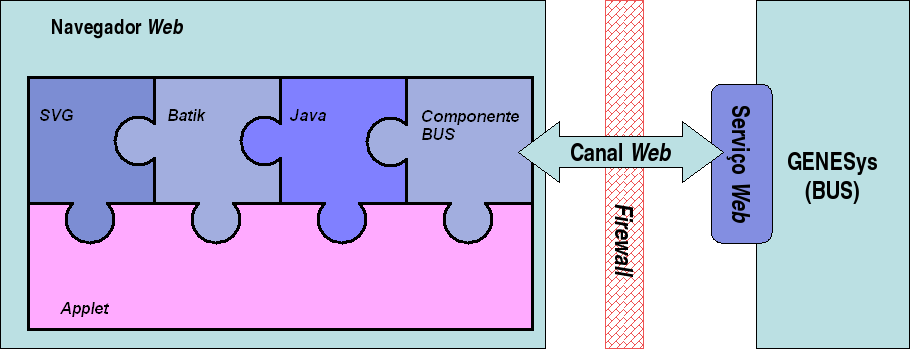
\includegraphics[width=0.86\textwidth]{puzzle}
    \caption{Arquitectura da Solução Proposta}
    \label{fig:arch}
  \end{center}
\end{figure}

Loren ipsum dolor sit amet, consectetuer adipiscing elit. 
Praesent sit amet sem. Maecenas eleifend facilisis leo. Vestibulum et
mi. Aliquam posuere, ante non tristique consectetuer, dui elit
scelerisque augue, eu vehicula nibh nisi ac est. Suspendisse elementum
sodales felis. Nullam laoreet fermentum urna. 

Duis eget diam. In est justo, tristique in, lacinia vel, feugiat eget,
quam. Pellentesque habitant morbi tristique senectus et netus et
malesuada fames ac turpis egestas. Fusce feugiat, elit ac placerat
fermentum, augue nisl ultricies eros, id fringilla enim sapien eu
felis. Vestibulum ante ipsum primis in faucibus orci luctus et
ultrices posuere cubilia Curae; Sed dolor mi, porttitor quis,
condimentum sed luctus. 

\subsection{Exemplo de Tabela}

É apresentado na Tabela~\ref{tab:exemplo1} um exemplo de tabela
flutuante e na Tabela~\ref{tab:exemplo2} um exemplo de tabela
flutuante, um pouco mais complicada.

\begin{table}[t]
  \centering
  \caption{Uma Tabela Simples}
\begin{tabular}{| l | p{45mm} |}
	\hline
\textbf{Acrónimo} & \textbf{Significado}\\
	\hline
	\hline
        ADT   & \emph{Abstract Data Type}\\\hline
        ANDF  & \emph{Architecture-Neutral Distribution Format}\\\hline
        API   & \emph{Application Programming Interface}\\
	\hline
\end{tabular}
  \label{tab:exemplo1}
\end{table}

Integer quis pede. Fusce nibh. Fusce nec erat vel mi condimentum
convallis. Sed at tortor non mauris pretium aliquet. In in lacus in
dolor molestie dapibus. Suspendisse potenti. Pellentesque sagittis
porta erat. Mauris sodales sapien id augue. Nam eu dolor. Donec sit
amet turpis non orci rhoncus commodo. Etiam condimentum commodo
libero.

Mauris pede. Curabitur faucibus dictum nibh. Proin tincidunt diam
vitae mauris. Sed hendrerit dolor vel ipsum. Nullam dapibus. Vivamus
tellus diam, egestas sit amet, vulputate non, vulputate id, eros. Nunc
sit amet nibh eget nibh imperdiet ornare. Cras vehicula mattis
ipsum. Sed diam arcu, semper at, gravida vitae, fermentum et,
nulla. Aenean massa orci, tristique nec, rutrum id, fringilla eget,
erat. Curabitur nulla ipsum, aliquam sed, rutrum vitae, semper quis,
ante. Fusce at nunc in dolor condimentum tempor. Duis sit amet massa. 

Curabitur convallis nulla quis risus. Nulla mollis porttitor
purus. Fusce ultricies odio at ligula pellentesque suscipit. Nulla
velit libero, blandit a, aliquet quis, hendrerit id, arcu. Phasellus
porttitor porttitor purus. Suspendisse velit tortor, fringilla sit
amet, commodo a, ultrices et, mi. Donec eu metus in erat ornare
adipiscing. Praesent varius mi ac nunc. Vestibulum leo lacus,
elementum in, vestibulum sit amet, hendrerit at, justo. Sed sit amet
neque. Donec libero risus, commodo sit amet, dignissim ut, tincidunt
a, eros. Ut non lacus quis tortor mattis ullamcorper. Vivamus
consequat augue vel erat. Sed tincidunt. Sed leo eros, ornare a,
pulvinar non, mattis quis, nibh. Aliquam faucibus mi ac nisi.

Pellentesque habitant morbi tristique senectus et netus et malesuada
fames ac turpis egestas. Duis aliquet, libero sit amet ornare viverra,
augue erat interdum dolor, vitae tincidunt lorem erat a lacus. Sed
lectus nisi, auctor in, hendrerit a, molestie vel, lectus. Cum sociis
natoque penatibus et magnis dis parturient montes, nascetur ridiculus
mus. Duis lacinia tempor dui. Vivamus rhoncus, tellus a viverra
dignissim, pede dui adipiscing odio, non faucibus metus mi gravida
eros. Nullam a tellus ut velit elementum tempus. Aenean rutrum
convallis tellus. Vestibulum nulla ante, dapibus ut, lobortis ut,
varius sed, nisl. Fusce lobortis. Sed ac lorem. Nulla tincidunt nulla
eget leo. Maecenas ac lectus eu neque ultrices pharetra. Curabitur a
risus nec arcu placerat tempor. Suspendisse magna nisl, viverra a,
adipiscing eget, ornare ultricies, ligula. Maecenas eu ligula vitae
eros convallis dignissim. 

\begin{table}[t]
  \centering
  \caption{Uma Tabela Mais Complicada}
\begin{tabular}{|c|r@{.}lr@{.}lr@{.}l||r|}
	\hline
\multicolumn{8}{|c|}
	{\rule[-3mm]{0mm}{8mm}Iteração $k$ de $f(x_n)$} \\
\textbf{\em k}
	& \multicolumn{2}{c}{$x_1^k$}
	& \multicolumn{2}{c}{$x_2^k$}
	& \multicolumn{2}{c||}{$x_3^k$}
	& comentários \\ \hline \hline
0   & -0&3                 & 0&6                 &  0&7   & - \\
1   &  0&47102965 & 0&04883157 & -0&53345964  & $\delta<\epsilon$ \\
2   &  0&49988691 & 0&00228830 & -0&52246185  & $\delta < \varepsilon$ \\
3   &  0&49999976 & 0&00005380 & -0&523656   &   $N$ \\
4   &  0&5                 & 0&00000307 & -0&52359743  & \\
\vdots	& \multicolumn{2}{c}{\vdots}
	& \multicolumn{2}{c}{$\ddots$}
	& \multicolumn{2}{c||}{\vdots}  & \\
7   &  0&5   & 0&0    & \textbf{-0}&\textbf{52359878}
		 & $\delta<10^{-8}$ \\ \hline
\end{tabular}
  \label{tab:exemplo2}
\end{table}

Loren ipsum dolor sit amet, consectetuer adipiscing elit. 
Praesent sit amet sem. Maecenas eleifend facilisis leo. Vestibulum et
mi. Aliquam posuere, ante non tristique consectetuer, dui elit
scelerisque augue, eu vehicula nibh nisi ac est. Suspendisse elementum
sodales felis. Nullam laoreet fermentum urna. 

Duis eget diam. In est justo, tristique in, lacinia vel, feugiat eget,
quam. Pellentesque habitant morbi tristique senectus et netus et
malesuada fames ac turpis egestas. Fusce feugiat, elit ac placerat
fermentum, augue nisl ultricies eros, id fringilla enim sapien eu
felis. Vestibulum ante ipsum primis in faucibus orci luctus et
ultrices posuere cubilia Curae; Sed dolor mi, porttitor quis,
condimentum sed luctus. 

\section{Secção Exemplo}

Loren ipsum dolor sit amet, consectetuer adipiscing elit. 
Praesent sit amet sem. Maecenas eleifend facilisis leo. Vestibulum et
mi. Aliquam posuere, ante non tristique consectetuer, dui elit
scelerisque augue, eu vehicula nibh nisi ac est. Suspendisse elementum
sodales felis. Nullam laoreet fermentum urna. 

Duis eget diam. In est justo, tristique in, lacinia vel, feugiat eget,
quam. Pellentesque habitant morbi tristique senectus et netus et
malesuada fames ac turpis egestas. Fusce feugiat, elit ac placerat
fermentum, augue nisl ultricies eros, id fringilla enim sapien eu
felis. Vestibulum ante ipsum primis in faucibus orci luctus et
ultrices posuere cubilia Curae; Sed dolor mi, porttitor quis,
condimentum sed luctus. 

\section{Resumo e Conclusões}

Resumir e apresentar as conclusões que se podem tirar no fim deste
capítulo.

\chapter{Implementação}\label{chap:chap4}

\section*{}

Este capítulo pode ser dedicado à apresentação de detalhes de nível
mais baixo relacionados com o enquadramento e implementação das
soluções preconizadas no capítulo anterior.
Note-se no entanto que detalhes desnecessários à compreensão do
trabalho devem ser remetidos para anexos.

Dependendo do volume, a avaliação do trabalho pode ser incluída neste
capítulo ou pode constituir um capítulo separado.

\section{Secção Exemplo}

%\todofigure{Inserir uma figura sobre o Map/Reduce}

Lorem ipsum dolor sit amet, consectetuer adipiscing elit. Integer
hendrerit commodo ante. Pellentesque nibh libero, aliquam at, faucibus
id, commodo a, velit. 
%\todoline{Escrever sobre o map/reduce}
Duis eleifend sem eget leo. Morbi in est. Suspendisse magna sem,
varius nec, hendrerit non, tincidunt quis, quam. Aenean congue. 
%\todolines{A short entry in the list of todos}{A very long todonote
%  that certainly will fill more than a single line in the list of
%  todos. Just to make sure let's add some more text.} 
Vivamus vel est sit amet sem iaculis posuere. Cras mollis, enim vel
gravida aliquam, libero nunc ullamcorper dui, ullamcorper sodales
lectus nulla sed urna. Morbi aliquet porta risus. 
Proin vestibulum ligula a purus. Maecenas a nulla. 
Maecenas mattis est vitae neque auctor tempus. Etiam nulla dui,
mattis vitae, porttitor sed, aliquet ut, enim. Cras nisl magna,
aliquet et, laoreet at, gravida ac, neque. Sed id est. Nulla dapibus
dolor quis ipsum rhoncus cursus. 

\section{Mais uma Secção}

Lorem ipsum dolor sit amet, consectetuer adipiscing elit. Quisque
purus sapien, interdum ut, vestibulum a, accumsan ullamcorper,
erat. Mauris a magna ut leo porta imperdiet. Donec dui odio, porta in,
pretium non, semper quis, orci. Quisque erat diam, pharetra vel,
laoreet ac, hendrerit vel, enim. Donec tristique luctus risus. Fusce
dolor est, eleifend id, elementum sit amet, varius vitae, neque. Morbi
at augue. Ut sem ligula, auctor vitae, facilisis id, pharetra non,
lectus. Nulla lacus augue, aliquam eget, sollicitudin sed, hendrerit
eu, leo. Suspendisse ac tortor. Mauris at odio. Etiam vehicula. Nam
lacinia purus at nibh. Aliquam fringilla lorem ac justo. Ut nec
enim. 
%\todoref{Citar Map/reduce}

Quisque ullamcorper. Aliquam vel magna. Sed pulvinar dictum
ligula. Sed ultrices dolor ut turpis. Vivamus sagittis orci malesuada
arcu venenatis auctor. Proin vehicula pharetra urna. Aliquam egestas
nunc quis nisl. Donec ullamcorper. Nulla purus. Ut suscipit lacus
vitae dui. Mauris semper. Ut eget sem. Integer orci. Nam vitae dui
eget nisi placerat convallis. 

\begin{lstlisting}[float,language=Java, label=src:mapreduce, caption=Example map and reduce functions for word counting]
map(String key, String value): 
// key: document name 
// value: document contents 
for each word w in value:
EmitIntermediate(w, "1");

reduce(String key, Iterator values):
// key: a word 
// values: a list of counts 
int result = 0;
for each v in values: 
result += ParseInt(v);

Emit(AsString(result))
\end{lstlisting}

Sed id lorem. Proin gravida bibendum lacus. Sed molestie, urna quis
euismod laoreet, diam dolor dictum diam, vitae consectetuer leo ipsum
id ante. Integer eu lectus non mauris pharetra viverra. In feugiat
libero ut massa. Morbi cursus, lorem sollicitudin blandit semper,
felis magna pellentesque lacus, ut rhoncus leo neque at tellus. Sed
mattis, diam eget eleifend tincidunt, ligula eros tincidunt diam,
vitae auctor turpis est vel nunc. In eu magna. Donec dolor metus,
egestas sit amet, ultrices in, faucibus sed, lectus. Etiam est enim,
vehicula pharetra, porta non, viverra vel, nunc. Ut non sem. Etiam nec
neque. 

\section{Resumo ou Conclusões}

Proin vehicula pharetra urna. Aliquam egestas
nunc quis nisl. Donec ullamcorper. Nulla purus. Ut suscipit lacus
vitae dui. Mauris semper. Ut eget sem. Integer orci. Nam vitae dui
eget nisi placerat convallis. 

\chapter{Conclusões e Trabalho Futuro} \label{chap:concl}

\section*{}

Deve ser apresentado um resumo do trabalho realizado e apreciada a
satisfação dos objetivos do trabalho, uma lista de contribuições
principais do trabalho e as direções para trabalho futuro.

A escrita deste capítulo deve ser orientada para a total compreensão
do trabalho, tendo em atenção que, depois de ler o Resumo e a
Introdução, a maioria dos leitores passará à leitura deste capítulo de
conclusões e recomendações para trabalho futuro.

\section{Satisfação dos Objetivos}

Lorem ipsum dolor sit amet, consectetuer adipiscing elit. Etiam non
felis sed odio rutrum ultrices. Donec tempor dolor. Vivamus justo
neque, tempus id, ullamcorper in, pharetra non, tellus. Praesent eu
orci eu dolor congue gravida. Sed eu est. Donec pulvinar, lectus et
eleifend volutpat, diam sapien sollicitudin arcu, a sagittis libero
neque et dolor. Nam ligula. Cras tincidunt lectus quis nunc. Cras
tincidunt congue turpis. Nulla pede velit, sagittis a, faucibus vitae,
porttitor nec, ante. Nulla ut arcu. Cras eu augue at ipsum feugiat
hendrerit. Proin sed justo eu sapien eleifend elementum. Pellentesque
habitant morbi tristique senectus et netus et malesuada fames ac
turpis egestas. Vivamus quam lacus, pharetra vel, aliquam vel,
volutpat sed, nisl. 

Nullam erat est, vehicula id, tempor non, scelerisque at,
tellus. Pellentesque tincidunt, ante vehicula bibendum adipiscing,
lorem augue tempor felis, in dictum massa justo sed metus. Suspendisse
placerat, mi eget molestie sodales, tortor ante interdum dui, ac
sagittis est pede et lacus. Duis sapien. Nam ornare turpis et
magna. Etiam adipiscing adipiscing ipsum. Fusce sodales nisl a
arcu. Cras massa leo, vehicula facilisis, commodo a, molestie
faucibus, metus. Suspendisse potenti. Duis sagittis. Donec porta. Sed
urna. Maecenas eros. Vivamus erat ligula, pharetra sit amet, bibendum
et, fermentum sed, dolor. Nullam eleifend condimentum nibh. Integer
leo nibh, consequat eget, mollis et, sagittis ac, felis. Duis viverra
pede in pede. Phasellus molestie placerat leo. Praesent at tellus a
augue congue molestie. Proin sed justo eu sapien eleifend
elementum. Pellentesque habitant morbi tristique senectus et netus et
malesuada fames ac turpis egestas. 

\section{Trabalho Futuro}

Lorem ipsum dolor sit amet, consectetuer adipiscing elit. Aliquam
tempor tristique risus. Suspendisse potenti. Fusce id eros. In eu
enim. Praesent commodo leo. Nullam augue. Pellentesque tellus. Integer
pulvinar purus a dui convallis consectetuer. In adipiscing, orci vitae
lacinia semper, sapien elit posuere sem, ac euismod ipsum elit tempus
urna. Aliquam erat volutpat. Nullam suscipit augue sed
felis. Phasellus faucibus accumsan est. 

Aliquam felis justo, facilisis sit amet, bibendum ut, tempus ac,
dolor. Sed malesuada. Nunc non massa. In erat. Nulla
facilisi. Phasellus blandit, est in accumsan cursus, libero augue
elementum leo, vitae auctor mauris nisl ac tortor. Cras porttitor
ornare elit. Fusce at lorem. Sed lectus tortor, vestibulum id, varius
a, condimentum nec, lectus. Maecenas in nisi et magna pretium
aliquam. Pellentesque justo elit, feugiat nec, tincidunt a, dignissim
vel, ipsum. Sed nunc. Vestibulum ante ipsum primis in faucibus orci
luctus et ultrices posuere cubilia Curae; Aliquam tempus rhoncus
leo. Donec neque quam, cursus sit amet, ultricies varius, semper non,
pede. Donec porttitor. Sed aliquet feugiat elit.  

\vspace*{12mm}

Lorem ipsum dolor sit amet, consectetuer adipiscing elit. Phasellus
tellus pede, auctor ut, tincidunt a, consectetuer in, felis. Mauris
quis dolor et neque accumsan pellentesque. Donec dui magna,
scelerisque mattis, sagittis nec, porta quis, nulla. Vivamus quis
nisl. Etiam vitae nisl in diam vehicula viverra. Sed sollicitudin
scelerisque est. Nunc dapibus. Sed urna. Nulla gravida. Praesent
faucibus, risus ac lobortis dignissim, est tortor laoreet mauris,
dictum pellentesque nunc orci tincidunt tellus. Nullam pulvinar, leo
sed vestibulum euismod, ante ligula elementum pede, sit amet dapibus
lacus tortor ac nisl. Morbi libero. Integer sed dolor ac lectus
commodo iaculis. Donec ut odio.  
 

%%----------------------------------------
%% Final materials
%%----------------------------------------

%% Bibliography
%% Comment the next command if BibTeX file not used
%% bibliography is in ``myrefs.bib''
\PrintBib{myrefs}

%% comment next 2 commands if numbered appendices are not used
\appendix
\chapter{Appendix} \label{sec:appendix}

\begin{table}
  \begin{tabular}{|c|p{0.8\textwidth}|c|}
  \hline
  open & http://www.mcgame.com/ & EMPTY\\ \hline
  type & //input[@id=query and @name=query and @type=text] & computer\\ \hline
  clickAndWait & //input[@type=submit] & EMPTY\\ \hline
  clickAndWait & //a[@class=active and @href=http://www.mcgame.com/de/account/login and contains(text(),'Login')] & EMPTY\\ \hline
  type & //input[@id=email and @name=email and @type=text] & banana\\ \hline
  type & //input[@id=password and @name=password and @type=password] & apple\\ \hline
  click & //input[@id=save\_login and @name=save\_login and @type=checkbox] & EMPTY\\ \hline
  clickAndWait & //input[@class=btn\_small grey and @name=commit and @type=submit] & EMPTY\\ \hline
  open & http://www.mcgame.com/ & EMPTY\\ \hline
  type & //input[@class=alarm\_amount and @name=alarm\_amount and @type=text] & dress\\ \hline
  clickAndWait & //a[@href=http://www.mcgame.com/de/store/game/10210253-watch-dogs-season-pass and contains(text(),'Watch Dogs Season Pass')] & EMPTY\\ \hline
  clickAndWait & //a[@href=http://www.mcgame.com/de/store/publishers and contains(text(),'Kataloge von Publishern')] & EMPTY\\ \hline
  clickAndWait & //a[@href=http://www.mcgame.com/de/store/publishers/1104-rokapublish] & EMPTY\\ \hline
  clickAndWait & //a[@href=http://www.mcgame.com/de and contains(text(),'Mac Spiele')] & EMPTY\\ \hline
  type & //input[@id=searchtextbox and @name=field-keywords and @title=Searchen and @type=text]	banana \\ \hline
  clickAndWait & //input[@class=nav-submit-input and @title=Go and @type=submit] & EMPTY\\ \hline 
  clickAndWait & //a[@href=http://www.mcgame.com/de/pages/about and contains(text(),'Uber McGame')] & EMPTY\\ \hline
  select & //select[@id=sort and @class=sort] & label=Price: Low to High \\ \hline
  clickAndWait & //a[@href=http://www.mcgame.com/de/store/publishers/1045-activision and contains(text(),'Activision')] & EMPTY\\ \hline
  clickAndWait & //a[@href=http://www.mcgame.com/de/help and contains(text(),'Hilfe \& Support')] & EMPTY\\ \hline
  clickAndWait & //a[@href=http://www.mcgame.com/de/store/publishers/1041-bethesda-softworks and contains(text(),'Bethesda Softworks')] & EMPTY\\ \hline
  clickAndWait & //a[@href=http://www.mcgame.com/de/store/publishers/1055-capcom and contains(text(),'Capcom')] & EMPTY\\ \hline
  clickAndWait & //a[@href=http://www.mcgame.com/de/store/mac/core and contains(text(),'Core Games')] & EMPTY\\ \hline
  clickAndWait & //a[@href=http://www.mcgame.com/de/store/offers and contains(text(),'Angebote')] & EMPTY\\ \hline
  clickAndWait & //a[@href=http://www.mcgame.com/de/store/game/10470030-hitman-absolution-professional-edition and contains(text(),'Hitman Absolution: Professional Edition')] & EMPTY\\ \hline
  select & //select[@id=searchDropbox and @class=twotab and @onchange=this.parentForm.submit();] & label=Strategie \\ \hline
  clickAndWait & //a[@class=active and @href=https://www.mcgame.com/de/account/login and contains(text(),'Login')] & EMPTY\\ \hline
  clickAndWait & //a[@id=forgot\_password and @href=https://www.mcgame.com/reset/password and contains(text(),'Passwort vergessen?')] & EMPTY\\ \hline
  \end{tabular}
\caption{A full history file example.}
\label{tab:fullexec}
\end{table}

\lstset{language=XML,caption={An example of a .paradigm file with identified patterns},label=lst:paradigm_model}
\begin{lstlisting}
<?xml version="1.0" encoding="UTF-8"?>
<Paradigm:Model xmi:version="2.0"
 xmlns:xmi="http://www.omg.org/XMI"
 xmlns:Paradigm="http://www.example.org/Paradigm"
 title="http://www.mcgame.com/" >
  <nodes xsi:type="Paradigm:Init" name="Init" number="0"
  outgoingLinks="//@relations.0"/>
  
  <nodes xsi:type="Paradigm:Login" name="Login" number="1"
  incomingLinks="//@relations.0" outgoingLinks="//@relations.1">
    <configurations validity="Invalid" check="StayOnSamePage" >
     <inputs field="username" value="login"/>
      <inputs field="password" value="123abc"/>
    </configurations>
    <fields name="username" id="//input[@id=email and @name=email
    and @type=text]"/>
    <fields name="password" id="//input[@id=password and @name=password
    and @type=password]"/>
  </nodes>

  <nodes xsi:type="Paradigm:Call" name="Call" number="1"
  incomingLinks="//@relations.1" outgoingLinks="//@relations.2">
    <configurations />
    <field name="call_0" id="//a[@class=active
    and @href=http://www.mcgame.com/de/account/login
    and contains(text(),'Login')]"/>
  </nodes>
  
  <nodes xsi:type="Paradigm:Find" name="Search" number="2"
  incomingLinks="//@relations.2" outgoingLinks="//@relations.3">
    <configurations check="NumberOfResults_more_than"
    result="10" >
      <inputs field="find_0" value="computer"/>
    </configurations>
    <fields name="find_0" id="//input[@id=query and @name=query
    and @type=text]"/>
  </nodes>

  <nodes xsi:type="Paradigm:Sort" name="Sort" number="3"
  incomingLinks="//@relations.3" outgoingLinks="//@relations.4">
    <configurations check="alphabetically" position="">
      <inputs field="Price" value="100"/>
    </configurations>
    <fields name="Price" id="//select[@id=price]"/>
  </nodes>

  <nodes xsi:type="Paradigm:End" name="End" number="4" 2
  incomingLinks="//@relations.4"/>

  <relations xsi:type="Paradigm:Sequence" label=">>"
  source="//@nodes.0" destination="//@nodes.1"/> 6
  <relations xsi:type="Paradigm:Sequence" label=">>"
  source="//@nodes.1" destination="//@nodes.2"/> 8
  <relations xsi:type="Paradigm:Sequence" label=">>"
  source="//@nodes.2" destination="//@nodes.3"/> 10
  <relations xsi:type="Paradigm:Sequence" label=">>"
  source="//@nodes.3" destination="//@nodes.4"/> 12
</Paradigm:Model>
\end{lstlisting}

\lstset{caption={The result of LogProcessor executing with the content of Table \ref{tab:fullexec} as input. },label=lst:full_exec_proc}
\begin{lstlisting}
open 
typeSearch 
clickSubmit pageChange
clickLogin pageChange
typeEmail 
typePassword 
clickLogin 
clickSubmit pageChange
open 
type 
clickLink pageChange
clickLink pageChange
clickLink pageChange
clickLink pageChange
typeSearch 
clickSubmit pageChange
clickLink pageChange
selectSort 
clickLink pageChange
clickLink pageChange
clickLink pageChange
clickLink pageChange
clickLink pageChange
clickLink pageChange
clickLink pageChange
selectSubmit 
clickLogin pageChange
clickLink pageChange
\end{lstlisting}

\lstset{language=XML,caption={The default configuration loaded of there is no user-specified configuration},label=lst:default_config}
\begin{lstlisting}
<?xml version="1.0" encoding="UTF-8"?>
<conf>
	<!-- 
	    actions: number of actions the crawler will execute before stopping
	    redirections: number of redirects to the home page the crawler will do 
	       before stopping
	    politenessDelay: time to wait (in milliseconds) after each action
	    typedKeywords: list of words to insert in text input elements
		searchKeywords: regex with keywords that identify search elements
		sortKeywords: regex with keywords that identify sort elements
		loginKeywords: regex with keywords that identify login elements
		generalWordsToExclude: regex with keywords that mark elements that should not be 
		  accessed
		menuIdentifiers: list of ids/classes/names that identify menu elements
		masterIdentifiers: list of ids/classes/names that identify master elements 
		detailIdentifiers: list of ids/classes/names that identify detail elements 
		historyFilepath: specify absolute filepath for history file
		processedHistoryFilepath: specify absolute filepath for processed history file
		patternsFilepath: specify absolute filepath for PARADIGM model file
		patternsToFind: list of patterns that the explorer can search for. If "all" 
		  occurs, there will be no restriction.
		loginConfiguration: credentials for a correct login in the web app.
		tokenizerPatterns: patterns for LogProcessor
		includeChildrenNodesOnInteraction: boolean; on interaction with an input or 
		  select element, if children elements should be included  in the history file, 
		  but not interacted with.
	-->
	<actions>50</actions>
	<redirections>5</redirections>
	<politenessDelay>500</politenessDelay>
	<includeChildrenNodesOnInteraction>false</includeChildrenNodesOnInteraction>
	<searchKeywords>(input|select|textarea)(.*(=q|q(ue)?ry|s(ea)?rch|pesq(uisa)?|procura(r)?|busca(dor)?).*)</searchKeywords>
	<sortKeywords>((input|select|textarea).*sort)</sortKeywords>
	<loginKeywords>(user(name)?|pass(word)?|e?mail|(sign(ed)?(\\s|_)?(in|out)|log(ged)?(\\s|_)?(in|out)))</loginKeywords>
	<generalWordsToExclude>(buy|sell|mailto|add(\\s|_)?to(\\s|_)?cart|checkout)</generalWordsToExclude>
	<typedKeywords>
        <item>curtains</item>
        <item>coffee</item>
        <item>phone</item>
        <item>shirt</item>
        <item>computer</item>
        <item>dress</item>
        <item>banana</item>
        <item>sandals</item>
    </typedKeywords>
	<menuIdentifiers>
		<item>nav</item>
		<item>head</item>
		<item>menu</item>
		<item>top</item>
		<item>head</item>
		<item>foot</item>
	</menuIdentifiers>
	<masterIdentifiers>
		<item>refine</item>
		<item>relatedSearches</item>
		<item>spell</item>
		<item>category</item>
		<item>categories</item>
	</masterIdentifiers>
	<detailIdentifiers>
		<item>results</item>
		<item>searchResults</item>
		<item>entry</item>
	</detailIdentifiers>
	<historyFilepath>history.csv</historyFilepath>
	<processedHistoryFilepath>history.csv.processed</processedHistoryFilepath>
	<patternsFilepath>patterns.paradigm</patternsFilepath>
	<patternsToFind>
		<!-- item>All</item-->
		<item>Search</item>
		<item>Sort</item>
		<item>MasterDetail</item>
		<item>Call</item>
		<item>Input</item>
		<item>Login</item>
		<item>Menu</item>
	</patternsToFind>
	<!-- loginConfiguration>
		<username>user-name</username>
		<password>password</password>
	</loginConfiguration-->
	<tokenizerPatterns>
	    <patternEntry>
            <name>login</name>
            <regex>sign(ed)?(\\s|_)?(in|out)|log(ged)?(\\s|_)?(in|out)</regex>
        </patternEntry>
		<patternEntry>
			<name>submit</name>
			<regex>submit</regex>
		</patternEntry>
		<patternEntry>
			<name>homeLink</name>
			<regex>(home|main(\\s|_)?page|index|logo)</regex>
		</patternEntry>
		<patternEntry>
			<name>imageLink</name>
			<regex>link(.*)img|img(.*)link</regex>
		</patternEntry>
		<patternEntry>
			<name>nextLink</name>
			<regex>(link(.*)next|next(.*)link)</regex>
		</patternEntry>
		<patternEntry>
			<name>prevLink</name>
			<regex>(prev(ious)?(.*)link|link(.*)prev(ious)?)</regex>
		</patternEntry>
		<patternEntry>
			<name>firstLink</name>
			<regex>(first(.*)link)</regex>
		</patternEntry>
		<patternEntry>
			<name>lastLink</name>
			<regex>(link(.*)last)</regex>
		</patternEntry>
		<patternEntry>
			<name>languageLink</name>
			<regex>lang</regex>
		</patternEntry>
		<patternEntry>
			<name>buttonLink</name>
			<regex>href.*(button|btn)</regex>
		</patternEntry>
		<patternEntry>
			<name>searchResultLink</name>
			<regex>search.*result(.*row)?</regex>
		</patternEntry>
		<patternEntry>
			<name>link</name>
			<regex>link|href</regex>
		</patternEntry>
		<patternEntry>
			<name>option</name>
			<regex>option</regex>
		</patternEntry>
		<patternEntry>
			<name>username</name>
			<regex>user(\\s|_)?(name|id)?</regex>
		</patternEntry>
		<patternEntry>
			<name>verifyPassword</name>
			<regex>verify(\\s|_)?pass(word)?|pass(word)?(\\s|_)?confirm(ation)?</regex>
		</patternEntry>
		<patternEntry>
			<name>password</name>
			<regex>pass(word)?</regex>
		</patternEntry>
		<patternEntry>
			<name>email</name>
			<regex>e?mail</regex>
		</patternEntry>
		<patternEntry>
			<name>checkbox</name>
			<regex>checkbox</regex>
		</patternEntry>
		<patternEntry>
			<name>collapse</name>
			<regex>collapse</regex>
		</patternEntry>
		<patternEntry>
			<name>firstNameInput</name>
			<regex>(input|textarea).*first(\\s|_)?name</regex>
		</patternEntry>
		<patternEntry>
			<name>lastNameInput</name>
			<regex>(input|textarea).*last(\\s|_)?name</regex>
		</patternEntry>
		<patternEntry>
			<name>sort</name>
			<regex>((input|textarea|select).*sort)</regex>
		</patternEntry>
		<patternEntry>
			<name>search</name>
			<regex>(input|select|textarea)(.*(=q\\s|q(ue)?ry|s(ea)?rch|pesq(uisa)?|procura(r)?|busca(dor)?).*)</regex>
		</patternEntry>
		<patternEntry>
			<name>captcha</name>
			<regex>captcha</regex>
		</patternEntry>
		<patternEntry>
			<name>auth</name>
			<regex>auth</regex>
		</patternEntry>
		<patternEntry>
			<name>numberInput</name>
			<regex>number|price|quantity|qty\\s|zip(\\s|_)?code</regex>
		</patternEntry>
		<patternEntry>
            <name>button</name>
            <regex>button</regex>
        </patternEntry>
		<patternEntry>
			<name>clear</name>
			<regex>clear</regex>
		</patternEntry>
		<patternEntry>
            <name>input</name>
            <regex>\\/\\/(input|textarea).*text.*</regex>
        </patternEntry>
	</tokenizerPatterns>
</conf>
\end{lstlisting}

\lstset{language=XML,caption={The result of running the approach on Table \ref{tab:fullexec} and Listing \ref{lst:full_exec_proc}.},label=lst:full_pattern}
\begin{lstlisting}
<?xml version="1.0" encoding="UTF-8"?>
<Paradigm:Model xmi:version="2.0"
 xmlns:xmi="http://www.omg.org/XMI" xmlns:Paradigm="http://www.example.org/Paradigm"
title="http://www.mcgame.com/" >
	<nodes xsi:type="Paradigm:Init" name="Init" number="0" outgoingLinks="//@relations.0"/>
	<nodes xsi:type="Paradigm:Find" name="Find1" number="1" incomingLinks="//@relations.0" outgoingLinks="//@relations.1">
		<configurations check="NumberOfResults_more_than" Position="1" result="10" >
			<inputs  field="find_0" value="computer"/>
		</configurations>
		<fields name="find_0" id="//input[@id=query and @name=query and @type=text]"/>
	</nodes>
	<nodes xsi:type="Paradigm:Call" name="Call2" number="2" incomingLinks="//@relations.1" outgoingLinks="//@relations.2">
		<configurations />
		<field name="call_0" id="//a[@class=active and @href=http://www.mcgame.com/de/account/login and contains(text(),'Login')]"/>
	</nodes>
	<nodes xsi:type="Paradigm:Login" name="Login3" number="3" incomingLinks="//@relations.2" outgoingLinks="//@relations.3">
		<configurations validity="Invalid" check="StayOnSamePage" >
			<inputs  field="username" value="banana"/>
			<inputs  field="password" value="apple"/>
		</configurations>
		<fields name="username" id="//input[@id=email and @name=email and @type=text]"/>
		<fields name="password" id="//input[@id=password and @name=password and @type=password]"/>
	</nodes>
	<nodes xsi:type="Paradigm:Input" name="Input4" number="4" incomingLinks="//@relations.3" outgoingLinks="//@relations.4">
		<configurations value="dress" />
		<field name="input_0" id="//input[@class=alarm\_amount and @name=alarm\_amount and @type=text]"/>
	</nodes>
	<nodes xsi:type="Paradigm:Call" name="Call5" number="5" incomingLinks="//@relations.4" outgoingLinks="//@relations.5">
		<configurations />
		<field name="call_0" id="//a[@href=http://www.mcgame.com/de/store/game/10210253-watch-dogs-season-pass and contains(text(),'Watch Dogs Season Pass')]"/>
	</nodes>
	<nodes xsi:type="Paradigm:Call" name="Call6" number="6" incomingLinks="//@relations.5" outgoingLinks="//@relations.6">
		<configurations />
		<field name="call_0" id="//a[@href=http://www.mcgame.com/de/store/publishers and contains(text(),'Kataloge von Publishern')]"/>
	</nodes>
	<nodes xsi:type="Paradigm:Call" name="Call7" number="7" incomingLinks="//@relations.6" outgoingLinks="//@relations.7">
		<configurations />
		<field name="call_0" id="//a[@href=http://www.mcgame.com/de/store/publishers/1104-rokapublish]"/>
	</nodes>
	<nodes xsi:type="Paradigm:Call" name="Call8" number="8" incomingLinks="//@relations.7" outgoingLinks="//@relations.8">
		<configurations />
		<field name="call_0" id="//a[@href=http://www.mcgame.com/de and contains(text(),'Mac Spiele')]"/>
	</nodes>
	<nodes xsi:type="Paradigm:Find" name="Find9" number="9" incomingLinks="//@relations.8" outgoingLinks="//@relations.9">
		<configurations check="NumberOfResults_more_than" Position="1" result="10" >
			<inputs  field="find_0" value="banana "/>
		</configurations>
		<fields name="find_0" id="//input[@id=searchtextbox and @name=field-keywords and @title=Searchen and @type=text]"/>
	</nodes>
	<nodes xsi:type="Paradigm:Call" name="Call10" number="10" incomingLinks="//@relations.9" outgoingLinks="//@relations.10">
		<configurations />
		<field name="call_0" id="//a[@href=http://www.mcgame.com/de/pages/about and contains(text(),'Uber McGame')]"/>
	</nodes>
	<nodes xsi:type="Paradigm:Sort" name="Sort11" number="11" incomingLinks="//@relations.10" outgoingLinks="//@relations.11">
		<configurations />
			<inputs  field="sort_0" value="label=Price: Low to High "/>
		<fields name="sort_0" id="//select[@id=sort and @class=sort]"/>
	</nodes>
	<nodes xsi:type="Paradigm:Call" name="Call12" number="12" incomingLinks="//@relations.11" outgoingLinks="//@relations.12">
		<configurations />
		<field name="call_0" id="//a[@href=http://www.mcgame.com/de/store/publishers/1045-activision and contains(text(),'Activision')]"/>
	</nodes>
	<nodes xsi:type="Paradigm:Call" name="Call13" number="13" incomingLinks="//@relations.12" outgoingLinks="//@relations.13">
		<configurations />
		<field name="call_0" id="//a[@href=http://www.mcgame.com/de/help and contains(text(),'Hilfe \ Support')]"/>
	</nodes>
	<nodes xsi:type="Paradigm:Call" name="Call14" number="14" incomingLinks="//@relations.13" outgoingLinks="//@relations.14">
		<configurations />
		<field name="call_0" id="//a[@href=http://www.mcgame.com/de/store/publishers/1041-bethesda-softworks and contains(text(),'Bethesda Softworks')]"/>
	</nodes>
	<nodes xsi:type="Paradigm:Call" name="Call15" number="15" incomingLinks="//@relations.14" outgoingLinks="//@relations.15">
		<configurations />
		<field name="call_0" id="//a[@href=http://www.mcgame.com/de/store/publishers/1055-capcom and contains(text(),'Capcom')]"/>
	</nodes>
	<nodes xsi:type="Paradigm:Call" name="Call16" number="16" incomingLinks="//@relations.15" outgoingLinks="//@relations.16">
		<configurations />
		<field name="call_0" id="//a[@href=http://www.mcgame.com/de/store/mac/core and contains(text(),'Core Games')]"/>
	</nodes>
	<nodes xsi:type="Paradigm:Call" name="Call17" number="17" incomingLinks="//@relations.16" outgoingLinks="//@relations.17">
		<configurations />
		<field name="call_0" id="//a[@href=http://www.mcgame.com/de/store/offers and contains(text(),'Angebote')]"/>
	</nodes>
	<nodes xsi:type="Paradigm:Call" name="Call18" number="18" incomingLinks="//@relations.17" outgoingLinks="//@relations.18">
		<configurations />
		<field name="call_0" id="//a[@href=http://www.mcgame.com/de/store/game/10470030-hitman-absolution-professional-edition and contains(text(),'Hitman Absolution: Professional Edition')]"/>
	</nodes>
	<nodes xsi:type="Paradigm:Call" name="Call19" number="19" incomingLinks="//@relations.18" outgoingLinks="//@relations.19">
		<configurations />
		<field name="call_0" id="//a[@class=active and @href=https://www.mcgame.com/de/account/login and contains(text(),'Login')]"/>
	</nodes>
	<nodes xsi:type="Paradigm:Call" name="Call20" number="20" incomingLinks="//@relations.19" outgoingLinks="//@relations.20">
		<configurations />
		<field name="call_0" id="//a[@id=forgot\_password and @href=https://www.mcgame.com/reset/password and contains(text(),'Passwort vergessen?')]"/>
	</nodes>
	<nodes xsi:type="Paradigm:End" name="End" number="21" incomingLinks="//@relations.20"/>

	<relations xsi:type="Paradigm:Sequence" label=">>" source="//@nodes.0" destination="//@nodes.1"/>
	<relations xsi:type="Paradigm:Sequence" label=">>" source="//@nodes.1" destination="//@nodes.2"/>
	<relations xsi:type="Paradigm:Sequence" label=">>" source="//@nodes.2" destination="//@nodes.3"/>
	<relations xsi:type="Paradigm:Sequence" label=">>" source="//@nodes.3" destination="//@nodes.4"/>
	<relations xsi:type="Paradigm:Sequence" label=">>" source="//@nodes.4" destination="//@nodes.5"/>
	<relations xsi:type="Paradigm:Sequence" label=">>" source="//@nodes.5" destination="//@nodes.6"/>
	<relations xsi:type="Paradigm:Sequence" label=">>" source="//@nodes.6" destination="//@nodes.7"/>
	<relations xsi:type="Paradigm:Sequence" label=">>" source="//@nodes.7" destination="//@nodes.8"/>
	<relations xsi:type="Paradigm:Sequence" label=">>" source="//@nodes.8" destination="//@nodes.9"/>
	<relations xsi:type="Paradigm:Sequence" label=">>" source="//@nodes.9" destination="//@nodes.10"/>
	<relations xsi:type="Paradigm:Sequence" label=">>" source="//@nodes.10" destination="//@nodes.11"/>
	<relations xsi:type="Paradigm:Sequence" label=">>" source="//@nodes.11" destination="//@nodes.12"/>
	<relations xsi:type="Paradigm:Sequence" label=">>" source="//@nodes.12" destination="//@nodes.13"/>
	<relations xsi:type="Paradigm:Sequence" label=">>" source="//@nodes.13" destination="//@nodes.14"/>
	<relations xsi:type="Paradigm:Sequence" label=">>" source="//@nodes.14" destination="//@nodes.15"/>
	<relations xsi:type="Paradigm:Sequence" label=">>" source="//@nodes.15" destination="//@nodes.16"/>
	<relations xsi:type="Paradigm:Sequence" label=">>" source="//@nodes.16" destination="//@nodes.17"/>
	<relations xsi:type="Paradigm:Sequence" label=">>" source="//@nodes.17" destination="//@nodes.18"/>
	<relations xsi:type="Paradigm:Sequence" label=">>" source="//@nodes.18" destination="//@nodes.19"/>
	<relations xsi:type="Paradigm:Sequence" label=">>" source="//@nodes.19" destination="//@nodes.20"/>
	<relations xsi:type="Paradigm:Sequence" label=">>" source="//@nodes.20" destination="//@nodes.21"/>
</Paradigm:Model>

\end{lstlisting}

%% Index
%% Uncomment next command if index is required
%% don't forget to run ``makeindex mieic-en'' command
%\PrintIndex

\end{document}
